\documentclass[paper=a4, fontsize=11pt]{scrartcl}
\usepackage[T1]{fontenc}
\usepackage{fourier}

\usepackage[english]{babel}															% English language/hyphenation
\usepackage[protrusion=true,expansion=true]{microtype}	
\usepackage{amsmath,amsfonts,amsthm} % Math packages
\usepackage[pdftex]{graphicx}	
\usepackage{url}
\usepackage{amsmath,amsxtra,amssymb,latexsym, amscd,amsthm}
\usepackage{indentfirst}
\usepackage{color}
\usepackage[utf8]{vietnam}
\usepackage{amsmath}
\usepackage[mathscr]{eucal}
\usepackage{amsfonts}
\usepackage{graphics}
\graphicspath{ {./images/} }
\usepackage{listings,xcolor}
\usepackage{fancybox}
\usepackage{float}
\usepackage{longtable}
\usepackage{fancyhdr}
\pagestyle{fancy}
%%% Custom sectioning
\usepackage{sectsty}
\allsectionsfont{\textbf \normalfont\scshape}


%%% Custom headers/footers (fancyhdr package)
\usepackage{fancyhdr}
\pagestyle{fancyplain}
\fancyhead{}											% No page header
\fancyfoot[L]{}											% Empty 
\fancyfoot[C]{}											% Empty
\fancyfoot[R]{\thepage}									% Pagenumbering
\renewcommand{\headrulewidth}{0pt}			% Remove header underlines
\renewcommand{\footrulewidth}{0pt}				% Remove footer underlines
\setlength{\headheight}{13.6pt}


%%% Equation and float numbering
\numberwithin{equation}{section}		% Equationnumbering: section.eq#
\numberwithin{figure}{section}			% Figurenumbering: section.fig#
\numberwithin{table}{section}				% Tablenumbering: section.tab#


%%% Maketitle metadata
\newcommand{\horrule}[1]{\rule{\linewidth}{#1}} 	% Horizontal rule

\title{
	%\vspace{-1in} 	
	\usefont{OT1}{bch}{b}{n}
	\normalfont \normalsize \textsc{Trường đại học Thăng Long} \\
	\Large Đề ôn tập môn: \\
	\Large BẢO MẬT THÔNG TIN
}
\author{
	\normalfont 								\normalsize
	Nguyễn Tú Anh\\[-3pt]		\normalsize
	\today
}
\date{}


%%% Begin document
\begin{document}
	\maketitle
	\newpage
	\textbf{Đề 1}
	
	\paragraph{Câu 1:} Cho hệ mật $(X, K, Y)$ với:\\
	\begin{tabular}{ll}
		$X$: Nguồn tin có phân phối:& 
		\begin{tabular}{|c|c|c|c|}
			\hline 
			X     & $x_1$ & $x_2$ & $x_3$\\
			\hline 
			$P_X$ & $1/4$ & $1/2$ & $1/4$\\
			\hline 
		\end{tabular} \\\\
		$K$: Khóa có phân phối:& 
		\begin{tabular}{|c|c|c|c|}
			\hline 
			K     & $k_1$ & $k_2$ & $k_3$\\
			\hline 
			$P_K$ & $1/3$ & $1/3$ & $1/3$\\
			\hline 
		\end{tabular} \\\\ 
		$Y= E_K(X)$ cho theo bảng:	
		&
		\begin{tabular}{|c|c|c|c|}
			\hline 
			      & $x_1$ & $x_2$ & $x_3$\\
			\hline 
			$k_1$ & 1      & 3    & 2    \\
			\hline 
			$k_2$ & 3      & 2    & 1    \\
			\hline 
			$k_3$ & 2      & 3    & 1   \\
			\hline 
		\end{tabular}\\
	\end{tabular} 

	\begin{itemize}
		\item[a,] Tính $H(X)$, $H(Y)$, $H(K)$.
		\item[b,] Tính $H(X|Y)$, $H(Y|X)$ và cho biết giữa X và Y trong kênh trên có độc lập không? Giải thích?.
	\end{itemize}	
	
	\paragraph{Câu 2:}
	\begin{itemize}
		\item[a,] Mã hóa P= "network security" bằng phương pháp Vigenere với khóa K= Shannon
		\item[b,] Tính số khóa có thể của hệ mã trên, biết rằng chu kỳ $d$ của khóa phải thỏa mãn điều kiện $2 \leq d$ và $d$ là ước của độ dài của P= 15.
	\end{itemize}

	\paragraph{Câu 3:} A chọn $p= 13, q= 11, e= 7$. B chọn $p= 11, q= 17, e= 9$
	
	\begin{itemize}
		\item[a,] Tính các khóa bí mật $K_{RA}$, $K_{RB}$ của A, B tương ứng.
		\item[b,] Hãy giúp A mã hóa tin P= 3 theo cả 2 trường hợp mã chứng thực và mã bảo mật.
	\end{itemize}
	
	\paragraph{Câu 4:} Cho hệ chữ ký RSA: với $p= 13, q= 17, e= 7$.
	
	\begin{itemize}
		\item[a,] Xác định chữ ký trên bản tin P= 2.
		\item[b,] Cho biết khóa công khai $K_U$ và bí mật $K_R$ của hệ trên.
	\end{itemize}

	\paragraph{Câu 5:} A, B sử dụng phương pháp Diffie-Hellman để trao đổi khóa chung $K_{AB}$ với lựa chọn $p= 11$, $\alpha= 2$.
	
	\begin{itemize}
		\item[a,] Chứng minh rằng $\alpha$ là phần tử nguyên thủy của $Z_p^*= Z_{11}^*$.
		\item[b,] Nếu khóa công khai của A là $K_{UA}= 5$, hãy tìm khóa bí mật $K_{RA}$.
		\item[c,] Nếu khóa công khai của B là $K_{UB}= 3$, hãy tìm khóa chung $K_{AB}$.
	\end{itemize}

	\paragraph{Câu 6:} Cho giao thức mật mã được mô tả theo sơ đồ như hình bên:
	\begin{figure}[H]
		\centering
		\label{fig:sodobmtt}
		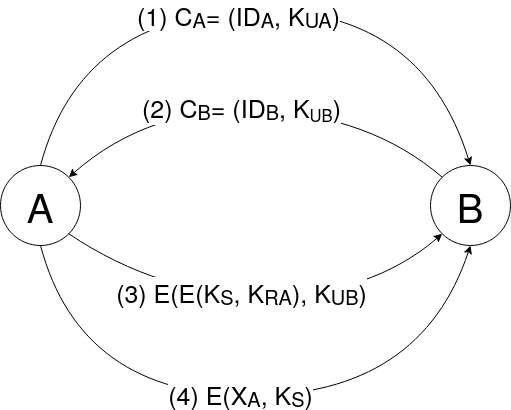
\includegraphics[width=0.7\linewidth]{SoDoBMTT}
	\end{figure}
	
	\begin{itemize}
		\item[a,] Hãy cho biêt giao thức trên là giao thức gì? Mục đích?
		\item[b,] Hãy giải thích các bước liên tiếp của giao thức? Mục địch?
		\item[c,] Để có thể xác thực được đối tượng (gửi, nhận) thì có cần bổ sung yêu cầu gì không? Giải thích?
		\item[d,] Giải thích vai trò của $K_S$.
	\end{itemize}
	
	\newpage
	\textbf{Đề 2}
	
	\paragraph{Câu 1:} Cho hệ mật $(X, K, Y)$ với:\\
	\begin{tabular}{ll}
		$X$: Nguồn tin có phân phối:& 
		\begin{tabular}{|c|c|c|c|}
			\hline 
			X     & $x_1$ & $x_2$ & $x_3$\\
			\hline 
			$P_X$ & $1/4$ & $1/4$ & $1/2$\\
			\hline 
		\end{tabular} \\\\
		$K$: Khóa có phân phối:& 
		\begin{tabular}{|c|c|c|c|}
			\hline 
			K     & $k_1$ & $k_2$ & $k_3$\\
			\hline 
			$P_K$ & $1/3$ & $1/3$ & $1/3$\\
			\hline 
		\end{tabular} \\\\ 
		$Y= E_K(X)$ cho theo bảng:	
		&
		\begin{tabular}{|c|c|c|c|}
			\hline 
			& $x_1$ & $x_2$ & $x_3$\\
			\hline 
			$k_1$ & 2      & 1    & 3    \\
			\hline 
			$k_2$ & 3      & 1    & 2    \\
			\hline 
			$k_3$ & 2      & 3    & 1   \\
			\hline 
		\end{tabular}\\
	\end{tabular} 
	
	\begin{itemize}
		\item[a,] Tính $H(X)$, $H(Y)$, $H(K)$.
		\item[b,] Tính $H(X|Y)$, $H(Y|X)$ và cho biết giữa X và Y trong kênh trên có độc lập không? Giải thích?.
	\end{itemize}	
	
	\paragraph{Câu 2:}
	\begin{itemize}
		\item[a,] Mã hóa P= "network security" bằng phương pháp Vigenere với khóa K= Maxtin.
		\item[b,] Tính số khóa có thể của hệ mã trên, biết rằng chu kỳ $d$ của khóa phải thỏa mãn điều kiện $2 \leq d$ và $d$ là ước của độ dài của P= 15.
	\end{itemize}
	
	\paragraph{Câu 3:} A chọn $p= 11, q= 13, e= 7$. B chọn $p= 17, q= 11, e= 13$
	
	\begin{itemize}
		\item[a,] Tính các khóa bí mật $K_{RA}$, $K_{RB}$ của A, B tương ứng.
		\item[b,] Hãy giúp A mã hóa tin P= 2 theo cả 2 trường hợp mã chứng thực và mã bảo mật.
	\end{itemize}
	
	\paragraph{Câu 4:} Cho hệ chữ ký RSA: với $p= 13, q= 17, e= 11$.
	
	\begin{itemize}
		\item[a,] Xác định chữ ký trên bản tin P= 3.
		\item[b,] Cho biết khóa công khai $K_U$ và bí mật $K_R$ của hệ trên.
	\end{itemize}
	
	\paragraph{Câu 5:} A, B sử dụng phương pháp Diffie-Hellman để trao đổi khóa chung $K_{AB}$ với lựa chọn $p= 13$, $\alpha= 2$.
	
	\begin{itemize}
		\item[a,] Chứng minh rằng $\alpha$ là phần tử nguyên thủy của $Z_p^*= Z_{11}^*$.
		\item[b,] Nếu khóa công khai của A là $K_{UA}= 7$, hãy tìm khóa bí mật $K_{RA}$.
		\item[c,] Nếu khóa công khai của B là $K_{UB}= 5$, hãy tìm khóa chung $K_{AB}$.
	\end{itemize}
	
	\paragraph{Câu 6:} Cho giao thức mật mã được mô tả theo sơ đồ:
	\begin{figure}[H]
		\centering
		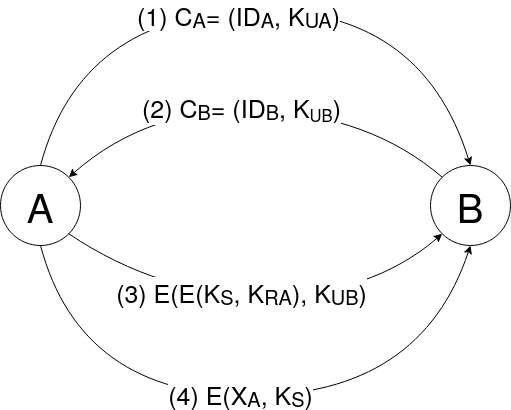
\includegraphics[width=0.7\linewidth]{SoDoBMTT}
		\label{fig:sodobmtt}
	\end{figure}
	
	\begin{itemize}
		\item[a,] Hãy cho biêt giao thức trên là giao thức gì? Mục đích?
		\item[b,] Hãy giải thích các bước liên tiếp của giao thức? Mục địch?
		\item[c,] Để có thể xác thực được đối tượng (gửi, nhận) thì có cần bổ sung yêu cầu gì không? Giải thích?
		\item[d,] Giải thích vai trò của $K_S$.
	\end{itemize}
	
\end{document}